\subsection{RQ2: What type of Fuzzing Algorithm is better for generating a Diverse test suite?}


One of the biggest advantages of fuzzing is that it can be customized to any domain with custom fuzzers, power schedules, and custom coverage or goal criterion.
% 
In RQ1, we observed that predicate coverage feedback outperforms code coverage feedback (Atheris) and no feedback (random fuzzing).
% 
In this section, we investigate whether changing the feedback or the power schedule would result in a change in coverage metric.
% 
To this end, we consider two of the most widely used power schedules in fuzzing, namely AFLFast and Entropic. 
% 
In contrast to AFLFast, Entropic can be provided with multiple coverage criterion as feedback.
% 
Our goal is to discover the most suitable power schedule and the feedback to improve the scenario coverage. 
%
We continue the experimental set up of RQ1, i.e., the same coverage metrics, mutators, seeds, and AV agents, and modify the power schedules and the feedback.


\subsubsection{Fuzzers}
\begin{itemize}
    \item PCGF-AFLFast.
    We implemented the AFLFast power schedule \cite{fuzzingbook2023:GreyboxFuzzer} and used it together with using predicate-sets for the fuzzing feedback.

    \item PCGF-Entropic.
    This is the fuzzer that we used for RQ1.

    \item PCGF-Entropic-MixedFeedback
    The Entropic power schedule allows having a fuzzing feedback that is comprised of several features of different types\footnote{These feature types are called \emph{species} in the Entropic paper.}.
    %
    Since our goal is to increase the total number of unique predicate valuations, in addition to the set of predicates, we also give the individual predicates as fuzzing feedback.

\end{itemize}



\begin{figure}
    \centering
    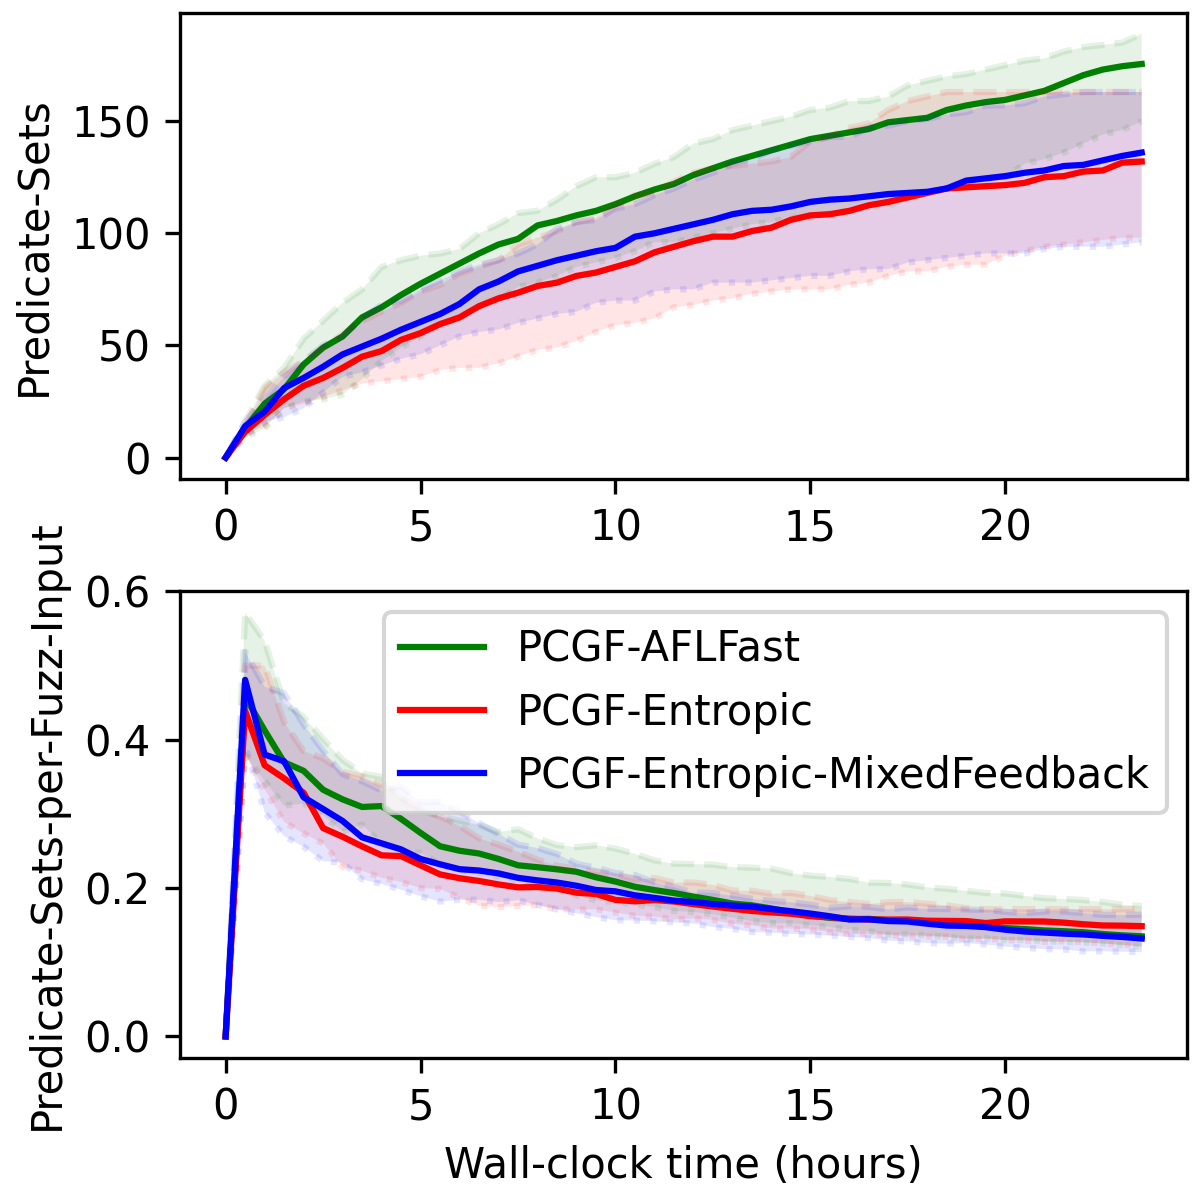
\includegraphics[width=0.6\linewidth]{figures/chapter5/RQ2/(PCGF-AFLFast,PCGF-Entropic,PCGF-Entropic-MixedFeedback)_TFPP_all-coverage_(Predicate-Sets,Predicate-Sets-per-Fuzz-Input).png}
    \caption{RQ2, TF++ agent.}
    \label{fig:RQ2-TFPP}
\end{figure}


\begin{figure}
    \centering
    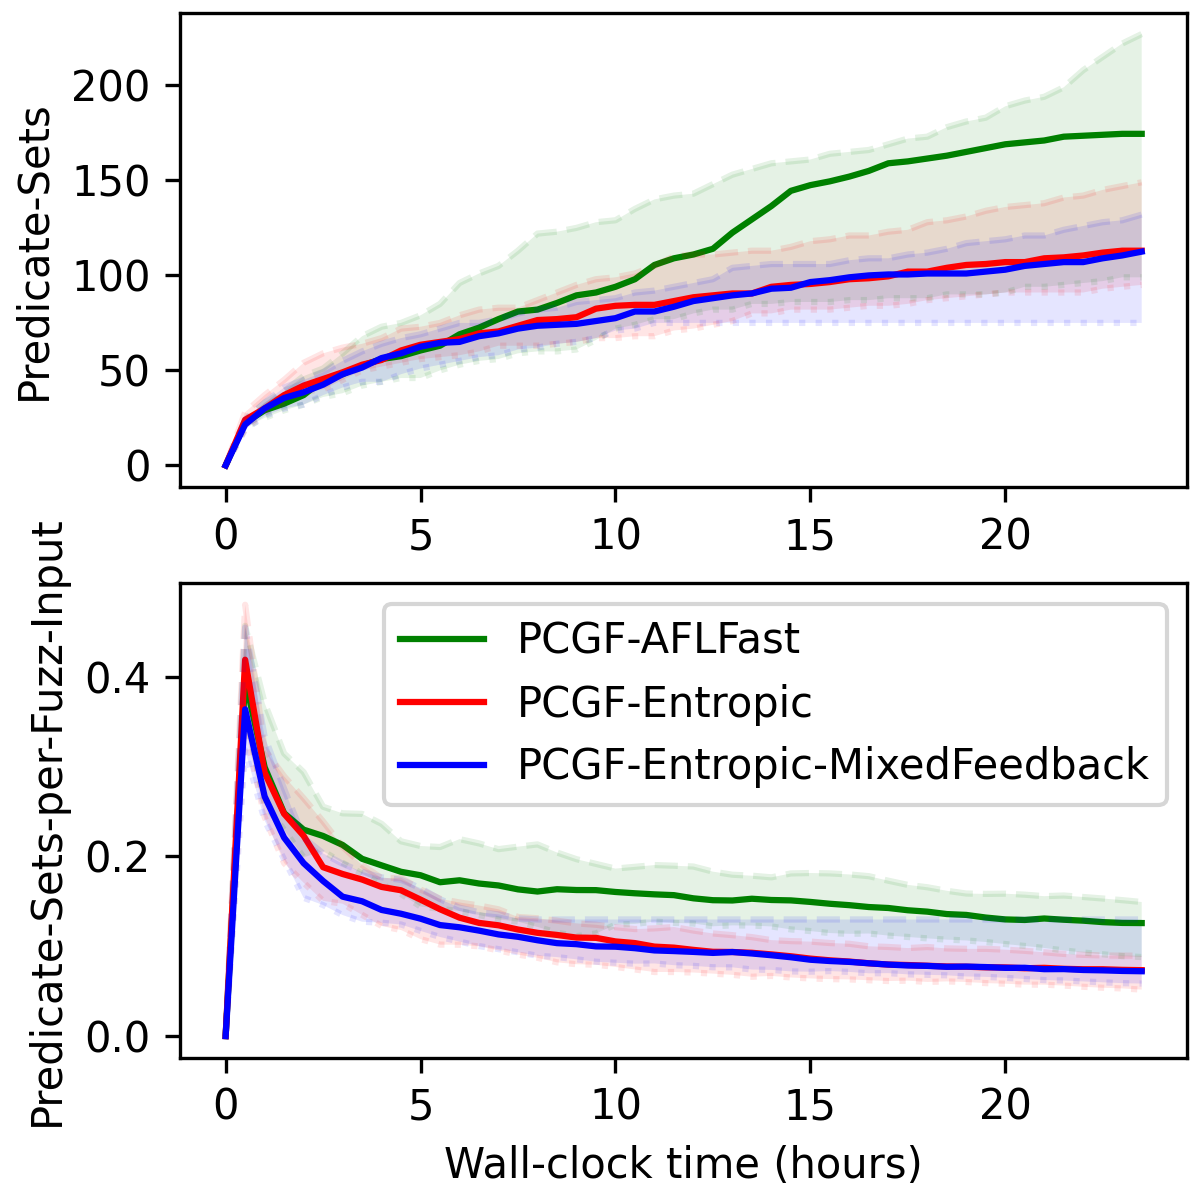
\includegraphics[width=0.6\linewidth]{figures/chapter5/RQ2/(PCGF-AFLFast,PCGF-Entropic,PCGF-Entropic-MixedFeedback)_autopilot_all-coverage_(Predicate-Sets,Predicate-Sets-per-Fuzz-Input).png}
    \caption{RQ2, CARLA Autopilot agent.}
    \label{fig:RQ2-autopilot}
\end{figure}


\begin{figure}
    \centering
    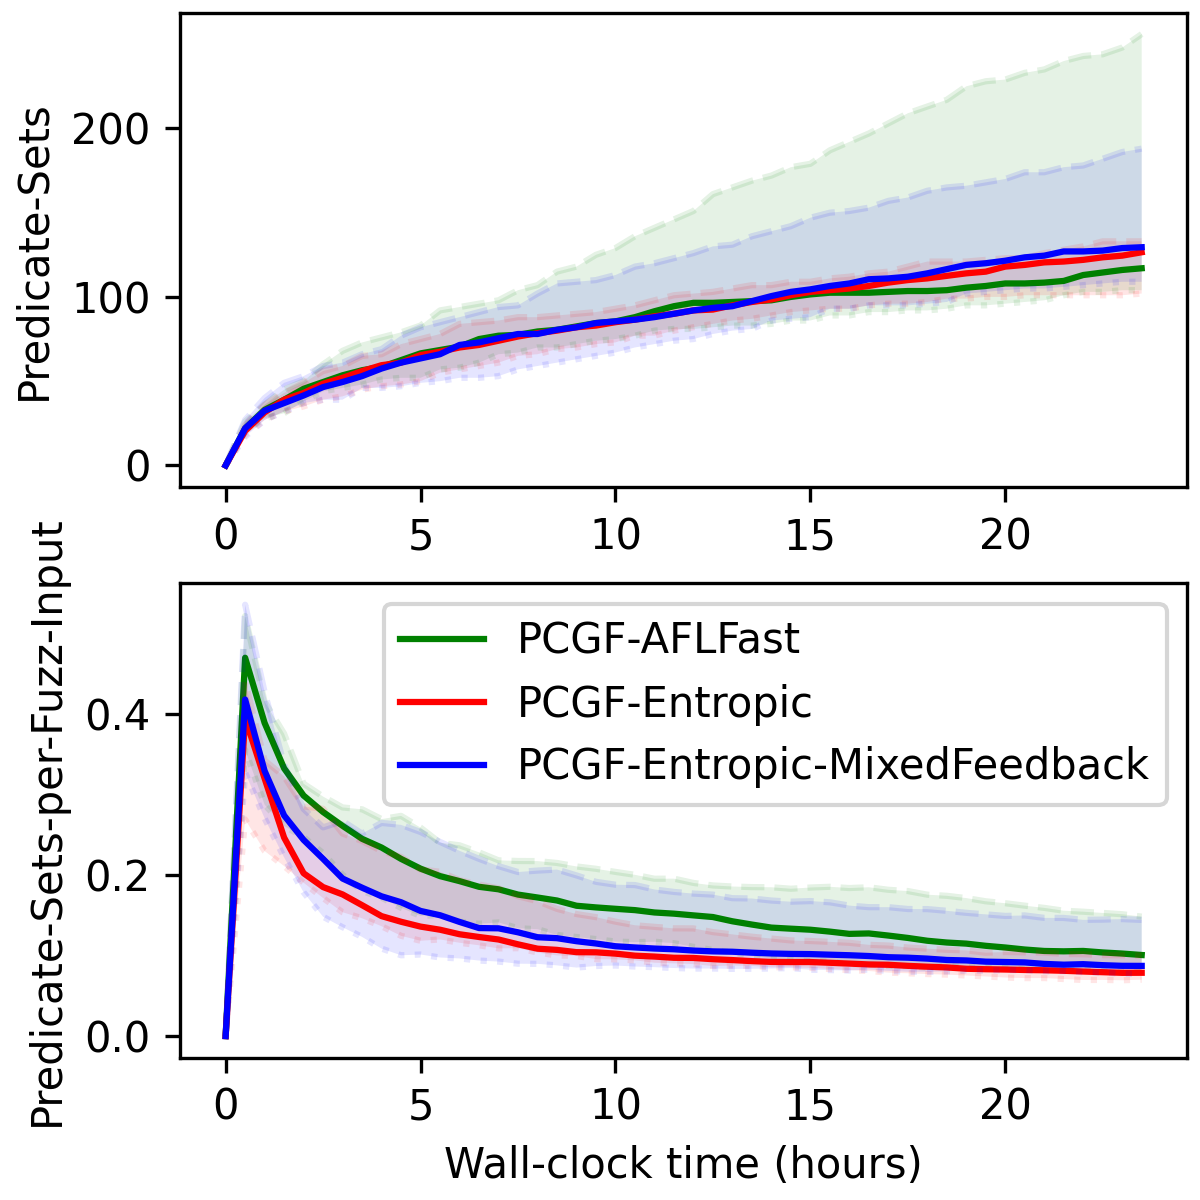
\includegraphics[width=0.6\linewidth]{figures/chapter5/RQ2/(PCGF-AFLFast,PCGF-Entropic,PCGF-Entropic-MixedFeedback)_BehaviorAgent_all-coverage_(Predicate-Sets,Predicate-Sets-per-Fuzz-Input).png}
    \caption{RQ2, CARLA BehaviorAgent agent.}
    \label{fig:RQ2-BehaviorAgent}
\end{figure}


\begin{figure}
    \centering
    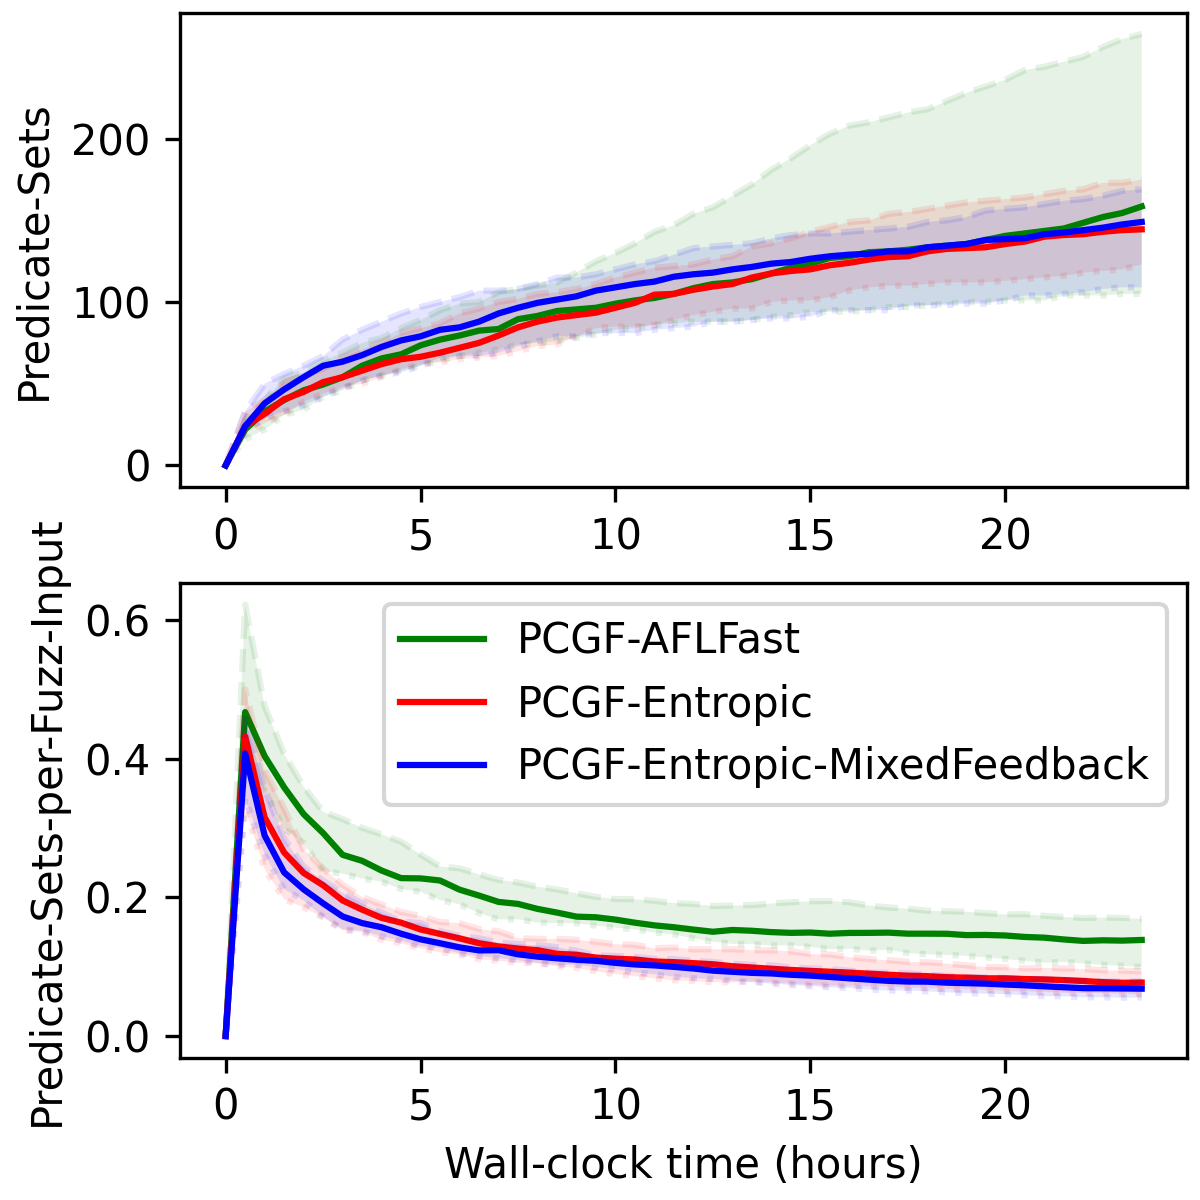
\includegraphics[width=0.6\linewidth]{figures/chapter5/RQ2/(PCGF-AFLFast,PCGF-Entropic,PCGF-Entropic-MixedFeedback)_intersectionAgent_all-coverage_(Predicate-Sets,Predicate-Sets-per-Fuzz-Input).png}
    \caption{RQ2, SCENIC agent.}
    \label{fig:RQ2-SCENICAgent}
\end{figure}


%---------------------
\subsubsection{Results}

Similar to RQ1, the evolution of coverage and coverage per fuzz input with time for all the techniques and all agents are given in Figures~\ref{fig:RQ2-TFPP},~\ref{fig:RQ2-autopilot},~\ref{fig:RQ2-BehaviorAgent},~\ref{fig:RQ2-SCENICAgent}.
% 
We draw two conclusions from these figures: 1) AFLFast achieves better coverage for all agents than both the version of Entropic and 2) Supplementing the predicate sets with the individual predicates as feedback does not result in any significant improvement for Entropic.
% 
% Our primary observation is that AFLFast achieves better coverage for all agents than both versions of Entropic.
% 
% Our secondary observation is that supplementing Entropic with additional coverage information does not improve the coverage performace.
%


The difference between AFLFast and other fuzzers is more pronounced in TF++ and Autopilot.
%
Also notice that the reason for AFLFast achieving better coverage is not because it generates more test cases.
% 
AFLFast outperforms other fuzzers in the coverage-per-fuzz-input metric too.
% 
The advantage of AFLFast over Entropic is contrary to our intuition as we expected the simplicity of AFLFast to come with a price.
%
The authors could not think of a reason for this clear improvement in performance of AFLFast; we would be glad if informed reviewers who are domain experts in fuzzing can help us in this regard.


The authors did not anticipate such a difference in coverage as a result of changing the power schedule.
% 
This surprising result might indicate that our platform can be a good candidate for benchmarking different fuzzing algorithms.
% 
% Furthermore, our experiments might provide a good benchmark for comparing fuzzing algorithms.


